\documentclass[11pt]{article}
\usepackage[a4paper,margin=1in]{geometry}
\usepackage[T1]{fontenc}
\usepackage{lmodern,microtype}
\usepackage{amsmath,amssymb,amsthm}
\usepackage{booktabs,array}
\usepackage{xcolor,listings}
\usepackage{needspace}
\usepackage{tikz}
\usetikzlibrary{positioning,arrows.meta}
\usepackage[hyphens]{url}
\usepackage[hidelinks]{hyperref}
\definecolor{codegray}{gray}{0.96}
\lstset{language=C++,basicstyle=\ttfamily\small,backgroundcolor=\color{codegray},
 frame=single,framerule=0.2pt,columns=fullflexible,keepspaces=true,
 breaklines=true,showstringspaces=false,tabsize=4}
\newcommand{\csolv}{\textsc{CSOLV}}
\newcommand{\jsolv}{\textsc{JSOLV}}
\newtheorem{proposition}{Proposition}
\title{CSOLV: C++ Static Object Labelling for Verification\\
Application-Owned Value-State Contracts in Standard C++}
\author{Jayanta Majumder \and Sambuddha Majumder}
\date{10 October 2026}
\begin{document}
\maketitle
\begin{abstract}
Nominal types describe what an object is, but often leave unstated whether it
has passed the workflow stages required by a consumer. An article can remain
an article while acquiring independent facts such as Persisted, Validated and
Authenticated. CSOLV, C++ Static Object Labelling for Verification, makes such
facts explicit and checks their use during ordinary standard C++17 compilation.
An application declares its label vocabulary in a two-key configuration file;
a build-time generator produces empty label types. A header-only library
represents known evidence in an owning value-state type and expresses consumer
requirements as borrowed parameter views. Establishment introduces trusted
facts, preservation unions existing and new facts, transformation discards old
evidence, selective revocation removes facts, and explicit selection retains
the intersection of branch evidence. The native compiler enforces membership
requirements, without a compiler plugin or vendor attributes. This paper
describes the design, its finite-set semantics, a complete application pattern,
build integration and diagnostics, and the boundaries of its guarantees. In
particular, checking declared evidence is distinct from proving business
predicates, deep immutability or borrowing lifetimes.
\end{abstract}

\section{Objects and the facts needed to use them}
Consider a publishing workflow. Persistence, title validation and author
authentication are independent preconditions for publication. Modelling each
combination as a new domain class obscures the stable identity of the domain
concept and scales poorly as the vocabulary grows. Runtime flags can express
the combination, but allow an incorrectly ordered workflow to reach production
before its mistake is detected.

The alternative is to keep the domain type \texttt{Article} and attach a finite
set of evidence labels to a value. A consumer declares the subset it needs.
Extra evidence is harmless, while missing evidence makes the call unacceptable.
The earlier static-property and semantic-role manuscripts motivate separating
such facts from nominal classes~\cite{tags,roles}. \jsolv{} implements this
idea for Java with generated annotations and a compiler processor~\cite{jsolv}.
The present sequel is self-contained: it develops the C++ interface and its
semantics without assuming familiarity with those implementations.

\csolv{} aims to make the vocabulary application-owned, contracts readable in
public interfaces, and enforcement active in an ordinary compiler build. It
does not attempt to infer every property of arbitrary C++ code. Its central
choice is to encode evidence in standard template types rather than attach
custom attributes whose interpretation depends on a compiler extension.

\section{Why standard syntax is not enough}
C++ provides the familiar \texttt{[[...]]} attribute syntax. However, an
implementation does not acquire the semantics of an application-defined label
merely by parsing an attribute: unrecognised attributes are ignored under the
language rules~\cite{attributes}. Thus a declaration decorated with
\texttt{[[csolv::Validated]]} cannot, by itself, cause every standard compiler
to check a validation precondition.

A compiler-specific frontend could interpret custom attributes and analyse
flow. That is a possible future frontend, but it brings compiler integration
and an effect model for mutation, aliases and calls. A textual scanner is no
substitute for a C++ frontend: preprocessing, overload resolution and template
instantiation determine what a program means.

\csolv{} instead uses ordinary templates and compile-time assertions, facilities
already supplied by C++~\cite{templates,assertions}. The header is the checking
library and the compiler is its enforcement engine. No optional external
analysis must run for the contracts to remain active. A Python checker driver
is included for convenient syntax-only compilation and JSON diagnostic capture;
it orchestrates the compiler rather than implementing a second C++ analyser.

\section{Architecture and application-owned vocabulary}
The implementation consists of four cooperating parts: a properties-to-header
generator, a portable C++17 header, a CMake integration helper, and an optional
compiler driver. A separate application owns its domain objects and evidence
vocabulary. Figure~\ref{fig:architecture} shows the build sequence.

\begin{figure}[ht]
\centering
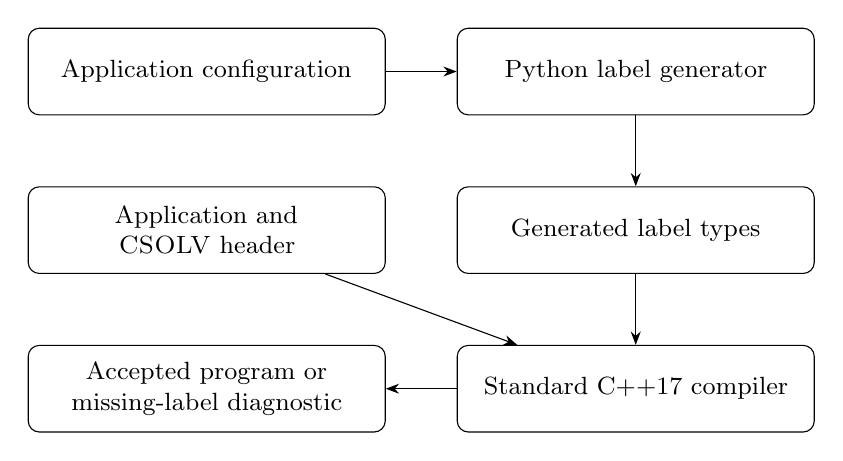
\begin{tikzpicture}[node distance=9mm,
 box/.style={draw,rounded corners,align=center,font=\small,text width=43mm,minimum height=11mm},
 >={Stealth}]
\node[box] (config) {Application configuration};
\node[box,right=of config] (generate) {Python label generator};
\node[box,below=of generate] (header) {Generated label types};
\node[box,left=of header] (app) {Application and\ \csolv{} header};
\node[box,below=of header] (compiler) {Standard C++17 compiler};
\node[box,left=of compiler] (result) {Accepted program or\ missing-label diagnostic};
\draw[->] (config)--(generate);
\draw[->] (generate)--(header);
\draw[->] (header)--(compiler);
\draw[->] (app)--(compiler);
\draw[->] (compiler)--(result);
\end{tikzpicture}
\caption{Generation establishes names; the native type checker enforces contracts.}
\label{fig:architecture}
\end{figure}

The application configuration is deliberately small:
\begin{lstlisting}[language={}]
namespace=example::tags
labels=Persisted, Validated, Authenticated
\end{lstlisting}
The generated header contains ordinary declarations:
\begin{lstlisting}
#pragma once
#include <csolv/csolv.hpp>
namespace example::tags {
struct Persisted : ::csolv::label {};
struct Validated : ::csolv::label {};
struct Authenticated : ::csolv::label {};
}
\end{lstlisting}
The marker permits generic checking without a built-in list of names. Adding
\texttt{Approved} to the configuration introduces a fourth independent label
after rebuilding; no library or checker change is required. Namespace-qualified
C++ type identity distinguishes vocabularies: two labels named Validated in
different namespaces are distinct facts.

The generator rejects malformed or reserved identifiers, duplicates, repeated
or unknown keys, and missing configuration fields. It supports blank lines and
full-line comments, but does not implement the escape and continuation grammar
of Java properties. It emits one header in the build tree, and does not rewrite
unchanged content. Replacing the header also removes labels deleted from the
configuration. A failed generation stops the dependent build. Related public
interfaces should share a vocabulary; independently generated conflicting
definitions in the same namespace are unsupported.

\section{Value states and requirement views}
The owning representation is
\texttt{csolv::labelled<T, Labels...>}. It stores one \emph{const} domain value,
with no runtime label instances or label bitset. Its constructor is private;
the public operations provide the explicit evidence introduction points.
The wrapper exposes a const lvalue accessor, has no mutable accessor or
destructive extraction, and cannot be assigned another payload.

Consumer requirements use a borrowing representation:
\begin{lstlisting}
using ReadyArticle = csolv::required<Article,
    Persisted, Validated, Authenticated>;
void publish(ReadyArticle article);
\end{lstlisting}
A suitable owning value converts to this view only if it contains every
required label. The view stores a pointer to the domain value; passing it does
not copy the article. The callee sees exactly its declared evidence, regardless
of extra facts known to the caller. This makes public, non-template parameter
contracts possible across translation units. Generic stages can instead retain
the exact evidence type of their input.

This interface deliberately favours explicit state transitions. Each stage
produces a fresh binding, normally declared with \texttt{auto}; an existing
variable does not change its C++ type as workflow knowledge grows. Ordinary
control-flow joins are not analysed by an external processor. They are written
with the explicit selection operation described below.

\section{Finite-set semantics}
Let $\mathcal L$ be the application vocabulary and let $S\subseteq\mathcal L$
be the evidence set of a value. Write $\operatorname{State}(T,S)$ for an owner
and $\operatorname{View}(T,R)$ for a consumer requirement view. The basic call
rule is
\[
 \operatorname{State}(T,S)\longrightarrow\operatorname{View}(T,R)
 \quad\text{is admissible exactly when}\quad R\subseteq S.
\]
The library implements membership with template instantiation and a separate
assertion for each requested label. This gives diagnostics whose instantiation
context identifies the missing label type.

\begin{table}[ht]
\centering\small
\begin{tabular}{lll}
\toprule
Operation & Output evidence & Domain value behaviour\\
\midrule
\texttt{establish<R...>} & $R$ & Own raw value\\
\texttt{require<R...>} & unchanged & Borrow const value if $R\subseteq S$\\
\texttt{preserve<R...>} & $S\cup R$ & Same-type transformation\\
\texttt{transform<R...>} & $R$ & Transformation, possibly new type\\
\texttt{drop<R...>} & $S\setminus R$ & Copy with revoked evidence\\
\texttt{forget} & no evidence & Ordinary domain-value copy\\
\texttt{select} & $S_1\cap S_2$ & Copy selected same-type value\\
\bottomrule
\end{tabular}
\caption{Evidence operations. Introduction and preservation are trusted contracts.}
\label{tab:algebra}
\end{table}

\paragraph{Introduction.}
\texttt{establish<R...>(value)} creates evidence $R$ for an ordinary value.
This is an explicit trust boundary, to be placed after the application has
performed the corresponding work. It does not implement those business checks.
Direct establishment on another evidence wrapper is rejected; use the
preservation or transformation interface instead.

\paragraph{Preservation.}
\texttt{preserve<R...>(state,f)} invokes $f$ on the const underlying value and
unions its new evidence $R$ with $S$. The returned domain type must be the same
as the input domain type. The promise concerns facts about the returned value,
not object identity: returning a distinct object is allowed if all the retained
facts still hold. Same-type checking prevents an obvious category of accidental
cross-domain transfer, but does not prove that promise.

\paragraph{Transformation and revocation.}
\texttt{transform<R...>} invokes a transformation and retains only the explicitly
new labels $R$. With no template arguments, it drops all incoming evidence.
\texttt{drop<R...>} removes selected facts without changing the copied value.
Revocation is conservative even if the property remains true: it removes
permission to rely on that evidence. \texttt{forget} returns an independent
ordinary value copy, with no CSOLV contract attached.

\paragraph{Selection.}
\texttt{select(condition,left,right)} returns the chosen domain value with
only common evidence. Both operands already exist and have the same nominal
domain type; the operation is not a lazy branch evaluator. Even a constant
condition does not change its conservative intersection rule. A less checked
alternative cannot lend its missing facts to the result.

The factories deduplicate labels and preserve first-occurrence order for
deterministic template types. Different orders may still yield different
owning C++ types even when their mathematical sets agree; requirement views
use membership and accept either order. Atomic labels have no inferred
implications, negation, disjunction or parameterised policy semantics.

\begin{proposition}[Conditional preservation of evidence meaning]
Suppose each introduced label is true of its value, each preservation operation
retains all incoming facts and establishes its advertised additions, and the
represented values and their relevant external context do not subsequently
invalidate these facts. Then every admissible requirement view constructed by
the public operations has all its required facts.
\end{proposition}
\begin{proof}
Introduction satisfies the hypothesis. Preservation takes the union of facts
assumed true of its result. Transformation asserts only its newly established
facts. Revocation keeps a subset, and selection keeps facts true in either
alternative. Requirement conversion accepts only a subset of the resulting
evidence. Induction over these operations gives the claim.
\end{proof}
This is a conditional statement about the evidence calculus, not a theorem
that arbitrary accepted C++ code is memory-safe or that authentication occurred.

\Needspace{22\baselineskip}
\section{A complete workflow pattern}
The following program uses a generated vocabulary and is sufficient to compile
and run after generation. Its persistence and credential operations are small
demonstrations. A production application supplies its real domain actions at
the same evidence introduction boundaries.

\begin{lstlisting}
#include <csolv_labels.hpp>
#include <iostream>
#include <stdexcept>
#include <string>
#include <utility>
#include <vector>
using namespace example::tags;
struct Article { std::string title; };

auto persist(Article article) {
    static std::vector<Article> store; // in-process demo storage
    store.push_back(article);
    return csolv::establish<Persisted>(std::move(article));
}
template<class State> auto validate(const State& article) {
    return csolv::preserve<Validated>(article,
        [](const Article& value) {
            if (value.title.empty())
                throw std::invalid_argument("empty title");
            return value;
        });
}
template<class State>
auto authenticate(const State& article, const std::string& token) {
    return csolv::preserve<Authenticated>(article,
        [&](const Article& value) {
            if (token != "demo-author")
                throw std::invalid_argument("invalid credential");
            return value;
        });
}
void publish(csolv::required<Article,
             Persisted, Validated, Authenticated> article) {
    std::cout << article.get().title << '\n';
}
int main() {
    const auto saved = persist(Article{"A value-state workflow"});
    const auto checked = validate(saved);
    const auto ready = authenticate(checked, "demo-author");
    publish(ready);
    // publish(saved); // compile-time missing-label error
}
\end{lstlisting}

The generic validation stage receives the full evidence type, so it preserves
Persisted when adding Validated. Authentication similarly retains both earlier
labels. Throwing before returning produces no successful new state. If a
stage instead accepts a concrete \texttt{required<Article, Validated>} view,
only Validated is visible to preservation within that stage, even when a
caller has additional evidence. Use generic stages when retention of the full
caller evidence is part of the intended interface.

\Needspace{12\baselineskip}
Editing is intentionally expressed differently:
\begin{lstlisting}
const auto edited = csolv::transform(ready, [](const Article& a) {
    return Article{a.title + " revised"};
}); // no prior evidence survives
const auto joined = csolv::select(condition, checked, saved);
static_assert(csolv::has_label_v<decltype(joined), Persisted>);
static_assert(!csolv::has_label_v<decltype(joined), Validated>);
\end{lstlisting}
Editing the title could invalidate validation or the relationship to a stored
record. The explicit reset prevents the old evidence being used accidentally.
The selection retains Persisted, which both alternatives have, and loses
Validated, which only one has. These snippets belong after the corresponding
bindings in the workflow, with a declared Boolean \texttt{condition}.

\section{Building and reporting}
The repository separates the reusable tool and library in
\texttt{development\_tools/csolv} from the application in
\texttt{development\_tools/csolv-app}. The latter has a public workflow header,
a separately compiled implementation, a main program, and an intentionally
rejected example excluded from its successful build. Its configuration remains
in the application directory; generated output stays in the build tree.

An application can add generation with the following CMake pattern:
\begin{lstlisting}[language={}]
add_subdirectory(path/to/csolv csolv-build)
add_executable(my_app main.cpp)
csolv_generate_labels(my_app
    "${CMAKE_CURRENT_SOURCE_DIR}/csolv.properties")
\end{lstlisting}
The helper links the header-only target, exposes the generated include path
and makes compilation depend on generation. Its custom command depends on
both the properties file and generator, following CMake's generated-output
dependency model~\cite{cmake}. A library target can own the shared vocabulary
and propagate includes to consumers.

From the repository root, the example and tests are built with:
\begin{lstlisting}[language={}]
cmake -S development_tools/csolv-app \
  -B development_tools/csolv-app/build -DCSOLV_BUILD_TESTS=ON
cmake --build development_tools/csolv-app/build
ctest --test-dir development_tools/csolv-app/build \
  --output-on-failure
\end{lstlisting}
These shell line continuations are for POSIX shells; PowerShell users can put
each command on one line. Multi-configuration generators additionally select
the build and test configuration. Requirements are C++17, CMake 3.20 or newer,
and Python 3.10 or newer; using a pre-generated vocabulary with the header alone
does not require Python or CMake.

The standalone generator accepts \texttt{--config} and \texttt{--output}. The
checker accepts a compiler path, optional JSON report path, and the application's
source and include arguments after \texttt{--}. Its default GNU-style check
uses standard C++17 and syntax-only compilation with pedantic errors. An MSVC
style supplies the corresponding compiler options. Flags are passed as an
argument array rather than through shell evaluation.

The report records schema version, invocation, acceptance, exit status and raw
diagnostic streams. It does not contain an expression-level provenance graph
or a business-predicate proof certificate. Each relevant translation unit
must be checked with its actual build flags; the driver does not discover a
compilation database, link an executable or run the application. Enforcement
is equally active when using the compiler directly.

\section{Ownership and the boundaries of evidence}
Const ownership is a deliberate safeguard. A mutable accessor could change a
validated title while leaving its label type unchanged. Moving the payload
out of an ordinary movable wrapper could leave the source moved-from while
its type still advertised the old evidence. \csolv{} stores a const payload:
moving a copyable owner copies that payload and preserves the source value.
Creating the first owner from a raw value can still move into const storage.

The resulting policy has costs. Preservation typically copies a value;
selection, revocation and erasure require copying. A move-only value can be
initially owned using C++17 return-value elision, but copying operations and
generally moving that owner are unavailable. There is no promise of zero
runtime overhead. Static label metadata requires no runtime storage, while
the exact wrapper size and calling convention remain implementation-dependent.

A requirement view borrows its owner's lifetime. Direct borrowing from a
temporary owner is deleted, and \texttt{require} and the owning accessor reject
rvalues to prevent simple dangling references. Nevertheless, C++ has no borrow
checker here: returning a view into a local owner or retaining a view after its
owner is destroyed remains erroneous. Views are appropriate for synchronous
parameter passing, not unowned asynchronous storage.

Constness is shallow. Pointees of pointers, \texttt{mutable} members and values
reachable through other aliases can change. Authentication can expire,
database records can change, and concurrent actors can invalidate contextual
facts. Prefer self-contained immutable snapshots and narrowly scoped trusted
contracts. CSOLV does not prove alias effects, thread safety, persistence
durability, credential validity or the absence of undefined behaviour. A
programmer can deliberately assert false evidence or misuse C++ casts and
internal machinery; the library is not a security boundary against such code.

\section{Validation and comparison with the Java frontend}
The implementation is exercised by 21 regression tests using actual compiler
invocations. Positive cases cover accumulation, intersection, revocation,
deduplication, borrowed contracts, erased copies, domain-changing
transformations and initial move-only ownership. Negative cases cover missing
requirements, lost evidence after edits, direct wrapper construction,
mutation, assignment, temporary borrowing, and preservation across unrelated
nominal types. Runtime checks verify source retention after moves and the
selected domain value. Generator tests cover malformed configurations,
stable output and a fourth application label compiled without library changes;
driver tests check successful and rejected JSON reports.

The application, its separate workflow compilation and the full CMake test
run pass with GCC 13.3.0 on Windows. The implementation uses standard C++17,
and the driver provides options for other compiler families, but this is not
a claim of empirical validation on Clang or MSVC. Additional compiler CI is
an appropriate next step.

Both frontends share application-owned atomic labels, subset requirements and
trusted preservation. Their enforcement mechanisms and user experience differ:
\jsolv{} uses annotations on ordinary Java values and a processor that tracks
local evidence; \csolv{} uses explicit standard C++ state types and native
template checking. Java branch analysis corresponds to an explicit C++ state
selection here. C++ adds selective evidence revocation and const ownership,
but makes copying and borrowing trade-offs visible. Neither mechanism turns a
declared workflow fact into an independently proved business predicate.

\section{Conclusion}
\csolv{} provides a compact, extensible vocabulary and an explicit evidence
algebra enforced by an ordinary standard C++17 compiler. Application developers
manage labels in configuration, introduce facts at audited domain boundaries,
and state requirements in public parameter types. Its portability follows
from using existing type-system mechanisms, while its limits follow from the
meaning of trusted evidence, shallow constness and ordinary C++ lifetimes.
The implementation leaves room for richer policy algebras and an optional
attribute-based compiler frontend without requiring either to add a new label.

\begin{thebibliography}{9}
\raggedright
\bibitem{tags} S. Majumder and J. Majumder.
\emph{User-Defined Static Property Tags for Mainstream Programming Languages:
A Lightweight Flow-Sensitive Verification Layer}. Companion manuscript,
\texttt{static\_property\_tags.tex}.
\bibitem{roles} J. Majumder and S. Majumder.
\emph{Explicit Semantic Categories for More Legible Mainstream Programming Languages}.
Companion manuscript,
\texttt{semantic\_roles\_beyond\_class.tex}.
\bibitem{jsolv} J. Majumder and S. Majumder.
\emph{JSOLV: Java Static Object Labelling for Verification}.
Companion manuscript, \texttt{jsolv.tex}, 2026.
\bibitem{attributes} ISO C++ working draft.
Attribute syntax and semantics, [dcl.attr.grammar].
\url{https://eel.is/c++draft/dcl.attr.grammar}.
\bibitem{templates} ISO C++ working draft.
Templates, [temp]. \url{https://eel.is/c++draft/temp}.
\bibitem{assertions} ISO C++ working draft.
Declarations, [dcl.pre], static assertions.
\url{https://eel.is/c++draft/dcl.pre}.
\bibitem{cmake} Kitware. CMake documentation: \texttt{add\_custom\_command}.
\url{https://cmake.org/cmake/help/latest/command/add_custom_command.html}.
\end{thebibliography}
\end{document}
